% !TeX program = xelatex
% ============================================================
% 1986 年·上海卷·理工农医类 · 解析版
% 由 tools/make_editions.py 生成（重跑会覆盖本文件）；
% 题目/解析内容在 questions.tex / answers*.tex，勿在本文件内写内容。
% ============================================================
\documentclass[zihao=-4, a4paper]{ctexart}
% ============================================================
% common/preamble.tex —— 拆分版试卷项目 · 公共导言区
% 引擎：XeLaTeX；文档类 ctexart 由各版本壳文件自行声明
% 由合并书 math-gaokao-2017-2026/preamble.tex 改造而来：
%   - 页眉左右改为可重定义宏 \gkheadL / \gkheadR（各版本壳设置）
%   - hyperref 不再写死 pdftitle（壳内 \hypersetup 覆盖）
%   - 删除书籍专用的 \chaptermark 重定义与 \gkpaper 装配宏
% ============================================================

% ---------- 数学 ----------
\usepackage{amsmath}
\usepackage{amssymb}
\usepackage{mathtools}

% ---------- 绘图 ----------
\usepackage{tikz}
\usetikzlibrary{shapes.geometric, arrows.meta, calc, patterns, angles, quotes, positioning}
\usepackage{pgfplots}
\pgfplotsset{compat=1.18}

% ---------- 版面 ----------
\usepackage{geometry}
\usepackage{needspace}
\geometry{a4paper, margin=2.2cm, headheight=15pt}
% 紧凑版式（如印刷版）可在壳文件中于 \begin{document} 前再次调用 \geometry 覆盖
\usepackage{enumitem}
\setlist{itemsep=2pt, topsep=4pt, parsep=0pt}

% 中文与行内公式混排的断行弹性：
% emergencystretch 允许段落末路不通时追加伸展量；
% 降低二元/关系符罚分，允许行内长公式在 = 、+ 等处断行（否则整段外溢）
\emergencystretch=2em
\binoppenalty=700
\relpenalty=500
\usepackage{booktabs}      % 三线表
\usepackage[most]{tcolorbox}

% ---------- 选择题选项对齐 ----------
% tasks 宏包：\begin{gkopts}(列数) \task ... \end{gkopts}
% 自动等宽分栏，选项天然对齐；列数已由内容片段按选项长度写定（4/2/1）
\usepackage{tasks}
\settasks{label={}, label-width=0pt, item-indent=1.2em,
          column-sep=1em, after-item-skip=2pt, before-skip=2pt, after-skip=4pt}
\NewTasksEnvironment[style=itemize]{gkopts}[\task](4)

% ---------- 页眉页脚 ----------
\newcommand{\gkheadL}{}   % 左页眉：卷名（壳文件 \renewcommand 设置）
\newcommand{\gkheadR}{}   % 右页眉：版本名（壳文件 \renewcommand 设置）
\usepackage{fancyhdr}
\pagestyle{fancy}
\fancyhf{}
\fancyhead[L]{\small\gkheadL}
\fancyhead[R]{\small\gkheadR}
\fancyfoot[C]{\small —— 第 \thepage\ 页 ——}
\renewcommand{\headrulewidth}{0.4pt}

% ---------- 超链接（须最后加载）----------
\usepackage{hyperref}
\hypersetup{colorlinks=true, linkcolor=blue!55!black,
            bookmarksnumbered=true, unicode=true}

% ============================================================
% common/macros.tex —— 自定义命令与环境（题号、解析头、提示框等）
% 与合并书 math-gaokao-2017-2026/preamble.tex 的自定义段保持一致，
% 保证内容片段（questions.tex / answers.tex）在两个项目间可互换。
% ============================================================

% ---------- 试卷标识（壳文件 \renewcommand 设置，用于 label 命名空间）----------
\newcommand{\gkpaperid}{none}

% ---------- 题号 ----------
% 试题部分的题号：加粗编号 + 自动 \label{q:<卷id>:<题号>}
\newcommand{\gkti}[1]{\par\medskip\noindent
  \textbf{#1．}\phantomsection\label{q:\gkpaperid:#1}\ignorespaces}
% 多卷/分部重启题号时，#1 是唯一内部顺序号（交叉引用身份），#2 才是原卷显示题号。
\newcommand{\gktiwithlabel}[2]{\par\medskip\noindent
  \textbf{#2．}\phantomsection\label{q:\gkpaperid:#1}\ignorespaces}

% 解析部分的题头：小标题 + 回链到试题页
% （仅在题目与解析同文档的版本中回链有效；试题版不含解析头，无悬空引用）
\newcommand{\gksolhead}[2]{%
  \Needspace{3\baselineskip}\subsubsection*{第 #1 题\if\relax\detokenize{#2}\relax\else（#2）\fi}%
  \phantomsection\label{s:\gkpaperid:#1}%
  {\small\color{gray}（题目见第~\pageref{q:\gkpaperid:#1}~页）}\par\nopagebreak}
% 与 \gktiwithlabel 成对：显示原题号，但回链仍用唯一内部顺序号。
\newcommand{\gksolheadwithlabel}[3]{%
  \Needspace{3\baselineskip}\subsubsection*{第 #2 题\if\relax\detokenize{#3}\relax\else（#3）\fi}%
  \phantomsection\label{s:\gkpaperid:#1}%
  {\small\color{gray}（题目见第~\pageref{q:\gkpaperid:#1}~页）}\par\nopagebreak}

% ---------- 填空题空位 ----------
\newcommand{\gkblank}{\underline{\hspace{2.2em}}}

% ---------- 提示框 ----------
% 卷种提示 / 解析归属声明（醒目，浅黄）
\newtcolorbox{gknotice}{colback=yellow!8, colframe=orange!60!black,
  boxrule=0.5pt, arc=1.5pt, left=6pt, right=6pt, top=4pt, bottom=4pt,
  before skip=8pt, after skip=8pt}

% 方法提示 / 注（浅蓝，用于解析后的点评与题量说明）
\newtcolorbox{gktip}{colback=blue!4, colframe=blue!35!black,
  boxrule=0.4pt, arc=1.5pt, left=6pt, right=6pt, top=4pt, bottom=4pt,
  before skip=6pt, after skip=6pt, fontupper=\small}

% ---------- 答案行 ----------
% 解析中独立成段的"答案：X"用带底色的行呈现
\newcommand{\gkanswer}[1]{\par\smallskip\noindent
  \tcbox[width=\linewidth, tcbox width=auto limited,
         colback=green!6, colframe=green!35!black, boxrule=0.4pt,
         arc=1.5pt, left=4pt, right=4pt, top=2pt, bottom=2pt,
         nobeforeafter]{\textbf{#1}}\par\smallskip}

% ---------- 结构标题 ----------
% 结构标题后通常紧跟一个带 0.5\textheight 起始预留的解析题块；0.4 只够放标题，
% 会把下一题整体推到下一页，留下孤立的「二、填空题」等页尾标题。
\newcommand{\gkpart}[1]{\Needspace{0.6\textheight}\subsection*{#1}\nopagebreak}     % 标题 + 首题
% （一）必考题 / 解析小问标题：块式加粗段，可自动换行（\paragraph 的 run-in 版式会溢出）
\newcommand{\gksubpart}[1]{\Needspace{6\baselineskip}\par\medskip\noindent\textbf{#1}\par\nopagebreak\smallskip}

% 罗马数字Ⅰ-Ⅻ（U+2160）与圈号①②③（U+2460）划入 CJK 字符类，
% 用中文字体渲染——西文字体 Latin Modern 缺这些字形，否则整段静默丢字
\xeCJKDeclareCharClass{CJK}{"2160 -> "217F, "2460 -> "24FF}

% ============================================================
% common/questions_env.tex —— 题目 / 解析的语义包装环境
%
% questions.tex 中每道题包在 \begin{question}...\end{question} 里，
% answers.tex 中每题解析包在 \begin{answer}...\end{answer} 里；
% 题头排版仍由内容行中的 \gkti / \gksolhead 完成（见 macros.tex）。
%
% 环境本身不产生任何盒子或垂直间距（只引入一个 TeX 分组），
% 排版结果与不包裹时逐点一致。它的价值在于：
%   1. 给每道题一个机器可数的结构边界（校验脚本数环境数 = 题量）；
%   2. 为将来的条件编译留钩子——某版本可重定义环境实现按题取舍。
% ============================================================

% 环境不把整题装盒：题目与解析仍可自然跨页，但开始题块前必须为题面、
% 图形/表格或解析首段留出足够空间。仅保留 2 个 baseline 会让题干、
% 选项和图形在页边界处被拆开，形成不可打印的孤立内容；题目保留
% 0.15\textheight，在避免短题制造大段空白与避免题块拆分之间取平衡。
% 解析题块保留 0.5\textheight，以容纳“题面 + 图形/选项 + 首段解析”；
% 结构标题仍用更大的保留量；末页自然收尾由视觉复审判定。
\newenvironment{question}{\Needspace{0.15\textheight}}{}
\newenvironment{answer}{\Needspace{0.5\textheight}}{}

\renewcommand{\gkpaperid}{gk-1986-regular-shanghai-science}
\renewcommand{\gkheadL}{1986 年·上海卷·理工农医类 · 数学}
\renewcommand{\gkheadR}{解析版}
\hypersetup{pdftitle={1986 年·上海卷·理工农医类 数学 · 解析版}}
\begin{document}
\begin{center}
  {\Large\bfseries 1986 年·上海卷·理工农医类}\\[4pt]
  {\large 数学 · 解析版}
\end{center}
\medskip
\pdfbookmark[1]{试题}{sec:q}
% questions.tex —— 1986 年·上海卷·理工农医类 · 题目内容片段（无答案）
% 由 tools/generate_projects.py 依来源总账自 1986/1986_数学真题_上海理_试题.md 生成，勿手改（改源 MD 后重跑）


\begin{gktip}
\textbf{来源说明}：本题面依据固定源 PDF《1986 年上海市普通高等学校招生统一考试数学题与解答·理工农医类》PDF 第 1—3 页逐题转录。原卷页码为 30—32；PDF 第 4—5 页为解答页，右栏出现的文史类题目不属于本卷。固定源同时含答案表和解答页，以下解析仍以题面为唯一题源，并由本库独立复算。

\textbf{版式与异文说明}：第 9 题“幅角的主值”沿固定源选项及答案表采用的 $[0,2\pi)$ 区间约定转录。第 5 题的 $k$ 取实数、且“纯虚数”是否排除 0，按固定源解答的处理说明，不把隐含约定改写成题面条件。

\textbf{图形说明}：第 6 题和第 7 题题面中的图形依据固定源关系重绘为 TikZ 矢量图；第 7 题的 $AB=\sqrt7$ 按折叠后的空间距离理解。
\end{gktip}

\begin{question}
\gkti{1}（本题满分 40 分）本题共有 20 个小题，每一个小题都给出代号为 $A\text{、}B\text{、}C\text{、}D$ 的四个结论，其中有且只有一个结论是正确的。答题时，在答题纸上把代表正确结论代号的小圈按答题纸上的要求涂黑，每小题涂对得 2 分，不涂、涂错或涂黑的小圈数超过一个，则得零分。

（1） 平移坐标轴，把原点 $O(0,0)$ 移到 $O'(2,-1)$，则点 $(-1,-3)$ 在新坐标系中的坐标是\mbox{（　　）}

（A）$(3,2)$　　（B）$(-3,-2)$　　（C）$(-3,2)$　　（D）$(3,-2)$

（2） 下列三角关系式中不正确的是\mbox{（　　）}

（A）$\sin\alpha+\sin\beta=2\sin\frac{\beta+\alpha}{2}\cos\frac{\beta-\alpha}{2}$

（B）$\sin\alpha-\sin\beta=2\cos\frac{\beta+\alpha}{2}\sin\frac{\beta-\alpha}{2}$

（C）$\cos\alpha+\cos\beta=2\cos\frac{\beta+\alpha}{2}\cos\frac{\beta-\alpha}{2}$

（D）$\cos\alpha-\cos\beta=2\sin\frac{\beta+\alpha}{2}\sin\frac{\beta-\alpha}{2}$

（3） 在直角坐标系中，直线 $x+\sqrt3y+1=0$ 的倾角是\mbox{（　　）}

（A）$\frac\pi6$　　（B）$\frac\pi3$　　（C）$\frac{2\pi}3$　　（D）$\frac{5\pi}6$

（4） 函数 $y=2\operatorname{tg}\left(3x+\dfrac\pi6\right)$ 的最小正周期是\mbox{（　　）}

（A）$\frac\pi6$　　（B）$\frac\pi3$　　（C）$\frac\pi2$　　（D）$\frac{2\pi}3$

（5） 在空间中，下列命题中正确的是\mbox{（　　）}

（A）如果两直线 $a\text{、}b$ 与直线 $l$ 所成的角相等，那么 $a\parallel b$。

（B）如果两直线 $a\text{、}b$ 与平面 $\alpha$ 所成的角相等，那么 $a\parallel b$。

（C）如果直线 $l$ 与两平面 $\alpha\text{、}\beta$ 所成的角都是直角，那么 $\alpha\parallel\beta$。

（D）如果平面 $\gamma$ 与两平面 $\alpha\text{、}\beta$ 所成的二面角都是直二面角，那么 $\alpha\parallel\beta$。

（6） 当 $|x|\le1$ 时，$\arccos(-x)$ 等于\mbox{（　　）}

（A）$\pi-\arccos x$　　（B）$-\arccos x$　　（C）$\arccos x$　　（D）$\pi+\arccos x$

\Needspace{5\baselineskip}
（7） 极坐标方程

\nopagebreak[4]
\[
\rho=\frac5{2-4\cos\theta}
\]

所表示的曲线是\mbox{（　　）}

（A）椭圆　　（B）抛物线　　（C）双曲线　　（D）直线

（8） 下列双曲线方程中，以 $y=\pm\dfrac12x$ 为渐近线的是\mbox{（　　）}

（A）$\frac{x^2}{16}-\frac{y^2}{4}=1$

（B）$\frac{x^2}{4}-\frac{y^2}{16}=1$

（C）$\frac{x^2}{2}-y^2=1$

（D）$x^2-\frac{y^2}{2}=1$

（9） 复数 $\sqrt3-i$ 的幅角的主值是\mbox{（　　）}

（A）$\frac\pi6$　　（B）$\frac{5\pi}6$　　（C）$\frac{7\pi}6$　　（D）$\frac{11\pi}6$

（10） 等式 $\log_3x^2=2$ 成立是等式 $\log_3x=1$ 成立的\mbox{（　　）}

（A）充分但不是必要条件　　（B）必要但不是充分条件

（C）充分而且必要条件　　（D）既不充分又不必要的条件

（11） 在等比数列中，已知首项为 $\dfrac98$，末项为 $\dfrac13$，公比为 $\dfrac23$，则项数是\mbox{（　　）}

（A）3　　（B）4　　（C）5　　（D）6

（12） 已知定直线 $l$ 和 $l$ 外一定点 $A$，过点 $A$ 且与 $l$ 相切的圆的圆心轨迹是\mbox{（　　）}

（A）抛物线　　（B）双曲线　　（C）椭圆　　（D）直线

（13） 若 $\sin\dfrac\theta2=\dfrac35$，$\cos\dfrac\theta2=-\dfrac45$，则 $\theta$ 角的终边在\mbox{（　　）}

（A）第一象限　　（B）第二象限　　（C）第三象限　　（D）第四象限

（14） 下列不等式中正确的是\mbox{（　　）}

（A）$\sin\frac{5\pi}7>\sin\frac{4\pi}7$

（B）$\operatorname{tg}\frac{15\pi}8>\operatorname{tg}\left(-\frac\pi7\right)$

（C）$\sin\left(-\frac\pi5\right)>\sin\left(-\frac\pi6\right)$

（D）$\cos\left(-\frac{3\pi}5\right)>\cos\left(-\frac{9\pi}4\right)$

（15） 函数 $y=\lg\left(x+\sqrt{x^2+1}\right)$ 是\mbox{（　　）}

（A）奇函数而不是偶函数　　（B）偶函数而不是奇函数

（C）既不是奇函数也不是偶函数　　（D）既是奇函数又是偶函数

（16） $0<a<b<1$，下列不等式中正确的是\mbox{（　　）}

（A）$a^a<a^b$　　（B）$b^a<b^b$　　（C）$a^a<b^a$　　（D）$b^b<a^b$

（17） 正方体 $ABCD-A_1B_1C_1D_1$ 中，直线 $BC_1$ 与 $AC$\mbox{（　　）}

（A）相交且垂直　　（B）相交但不垂直

（C）异面且垂直　　（D）异面但不垂直

（18） 设复数 $z=a+bi$（$a,b\in\mathbb R$，且 $b\ne0$），则 $|z^2|$，$|z|^2$，$z^2$ 的关系是\mbox{（　　）}

（A）$|z^2|=|z|^2\ne z^2$　　（B）$|z^2|=|z|^2=z^2$

（C）$|z^2|\ne|z|^2=z^2$　　（D）$|z^2|\ne|z|^2\ne z^2$

（19） 过抛物线焦点 $F$ 的直线与抛物线相交于 $A\text{、}B$ 两点。若 $A\text{、}B$ 在抛物线准线上的射影分别是 $A_1\text{、}B_1$，则 $\angle A_1FB_1$ 等于\mbox{（　　）}

（A）$45^\circ$　　（B）$60^\circ$　　（C）$90^\circ$　　（D）$120^\circ$

\Needspace{5\baselineskip}
（20） 令

\nopagebreak[4]
\[
I=\{(x,y)\mid x,y\in\mathbb R\},
\]

\nopagebreak[4]
\[
A=\left\{(x,y)\middle|\frac{y-3}{x-2}=1,\ x,y\in\mathbb R\right\},
\qquad
B=\{(x,y)\mid y=x+1,\ x,y\in\mathbb R\},
\]

则 $\overline A\cap B$ 是\mbox{（　　）}

（A）$\overline A$　　（B）$B$　　（C）$\varnothing$　　（D）$\{(2,3)\}$

\end{question}
\begin{question}
\gkti{2}（本题满分 30 分）本题共有 10 个小题，每一个小题满分 3 分，只要求直接写出结果。

\Needspace{5\baselineskip}
（1） 若三点 $P_1\text{、}P_2$ 和 $P$ 在一条直线上，点 $P_1$ 和点 $P_2$ 在直角坐标系中的坐标分别为 $(0,-6)$ 和 $(3,0)$，且

\nopagebreak[4]
\[
\frac{\overline{P_1P}}{\overline{PP_2}}=-\frac12,
\]

则点 $P$ 的坐标是 $\underline{\hspace{2em}}$。

（2） 正方体的全面积是 6，则其内切球的体积是 $\underline{\hspace{2em}}$。

\Needspace{5\baselineskip}
（3） 计算下式：

\nopagebreak[4]
\[
\lim_{n\to\infty}\frac{1+3+5+\cdots+(2n-1)}{n(n+1)}
=\underline{\hspace{2em}}\text{。}
\]

\Needspace{5\baselineskip}
（4） 求一次项系数：

\nopagebreak[4]
\[
\left(\sqrt[3]{x}-\frac1{\sqrt{x}}\right)^8
\]

的展开式中，$x$ 的一次项的系数是 $\underline{\hspace{2em}}$。

\Needspace{5\baselineskip}
（5） 不等式组

\nopagebreak[4]
\[
\begin{cases}
\sqrt{x^2-9}\le4,\\
x>0
\end{cases}
\]

的解是 $\underline{\hspace{2em}}$。

（6） 轴截面是等边三角形的圆锥，它的侧面展开图扇形的圆心角的弧度数等于 $\underline{\hspace{2em}}$。

（7） 用 1、2、3、4 四个数字组成没有重复数字的四位奇数的个数是 $\underline{\hspace{2em}}$。

\Needspace{5\baselineskip}
（8） 已知 $\cos\theta=-\dfrac35$ 且 $\pi<\theta<\dfrac{3\pi}2$，则

\nopagebreak[4]
\[
\operatorname{ctg}\left(\theta-\frac\pi4\right)=\underline{\hspace{2em}}\text{。}
\]

\Needspace{5\baselineskip}
（9） 函数

\nopagebreak[4]
\[
y=\log_2\left(\log_{\frac12}x\right)
\]

的定义域是 $\underline{\hspace{2em}}$。

\Needspace{5\baselineskip}
（10） 直线 $l$ 的参数方程为

\nopagebreak[4]
\[
\begin{cases}
x=3+\dfrac48t,\\
y=-2+\dfrac38t,
\end{cases}
\]

过点 $(4,-1)$ 且与 $l$ 平行的直线在 $y$ 轴上的截距是 $\underline{\hspace{2em}}$。

\end{question}
\begin{question}
\gkti{3}（本题满分 7 分）设数列 $\{a_n\}$ 的前 $n$ 项和为

\nopagebreak[4]
\[
S_n=n^2+2n+4\qquad(n\in\mathbb N),
\]

（1） 写出这个数列的前 $3$ 项 $a_1,a_2,a_3$；

（2） 证明：数列 $\{a_n\}$ 除去首项后所成的数列 $a_2,a_3,a_4,\ldots$ 是等差数列。

\end{question}
\begin{question}
\gkti{4}（本题满分 7 分）设 $x>0,\ y>0$，证明不等式

\nopagebreak[4]
\[
(x^2+y^2)^{1/2}>(x^3+y^3)^{1/3}.
\]

\end{question}
\begin{question}
\gkti{5}（本题满分 12 分）本题共有 2 个小题，每个小题满分 6 分。已知 $k$ 为实数，复数

\nopagebreak[4]
\[
z=\cos\theta+i\sin\theta.
\]

（1） 当 $\theta$ 和 $k$ 分别取何值时，$z^3+k\overline z^{\,3}$ 是纯虚数；

（2） 当 $\theta$ 变化时，求 $|z^3+k\overline z^{\,3}|$ 的最大值和最小值。

\Needspace{0.4\textheight}
\end{question}
\begin{question}
\gkti{6}（本题满分 12 分）如果抛物线

\nopagebreak[4]
\[
y^2=px
\]

\Needspace{5\baselineskip}
和圆

\nopagebreak[4]
\[
(x-2)^2+y^2=3
\]

相交，它们在 $x$ 轴上方的交点为 $A$ 和 $B$，那么当 $p$ 为何值时，线段 $AB$ 的中点 $M$ 在直线 $y=x$ 上。
\nopagebreak[4]
\begin{center}% 1986 年上海卷理工农医类第 6 题：抛物线与圆
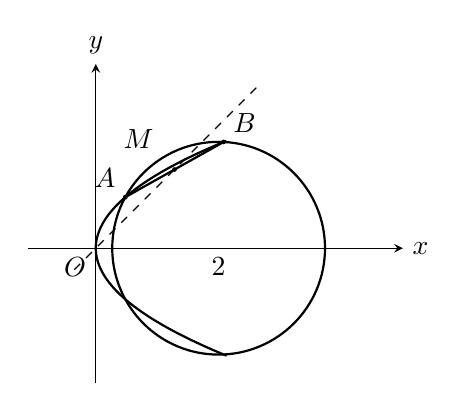
\begin{tikzpicture}[scale=0.78,>=stealth]
  \draw[->] (-1.1,0)--(5.0,0) node[right] {$x$};
  \draw[->] (0,-2.2)--(0,3.0) node[above] {$y$};
  \draw[thick] (2,0) circle (1.732);
  \draw[thick,domain=-1.75:1.75,samples=100]
    plot ({\x*\x/1.438},{\x});
  \draw[dashed] (-0.35,-0.35)--(2.65,2.65);
  \draw[thick] (0.480,0.831)--(2.081,1.730);
  \fill (0.480,0.831) circle (1.1pt) node[above left] {$A$};
  \fill (2.081,1.730) circle (1.1pt) node[above right] {$B$};
  \fill (1.281,1.281) circle (1.1pt) node[above left,xshift=-4pt,yshift=4pt] {$M$};
  \node[below left] at (0,0) {$O$};
  \node[below] at (2,0) {$2$};
\end{tikzpicture}
\end{center}
\nopagebreak[4]
\Needspace{0.4\textheight}
\end{question}
\begin{question}
\gkti{7}（本题满分 12 分）已知直角三角形 $ABC$ 的两直角边 $AC=2$，$BC=3$，$P$ 为斜边 $AB$ 上一点（图 1）。现沿 $CP$ 将此直角三角形折成直二面角 $A\mathbin{-}CP\mathbin{-}B$，当 $AB=\sqrt7$ 时，求二面角 $P\mathbin{-}AC\mathbin{-}B$ 的大小（图 2）。
\nopagebreak[4]
\begin{center}% 1986 年上海卷理工农医类第 7 题图 1：折叠前的直角三角形
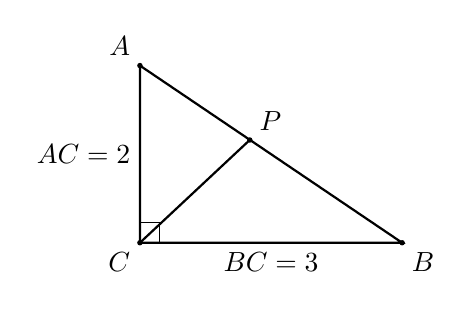
\begin{tikzpicture}[scale=0.9,>=stealth]
  \coordinate (C) at (0,0);
  \coordinate (A) at (0,2.5);
  \coordinate (B) at (3.7,0);
  \coordinate (P) at (1.55,1.45);
  \draw[thick] (A)--(C)--(B)--cycle;
  \draw[thick] (C)--(P);
  \draw (0,0.28)--(0.28,0.28)--(0.28,0);
  \fill (A) circle (1.1pt) node[above left] {$A$};
  \fill (B) circle (1.1pt) node[below right] {$B$};
  \fill (C) circle (1.1pt) node[below left] {$C$};
  \fill (P) circle (1.1pt) node[above right] {$P$};
  \node[left] at (0,1.25) {$AC=2$};
  \node[below] at (1.85,0) {$BC=3$};
\end{tikzpicture}
\end{center}
\nopagebreak[4]
\nopagebreak[4]
\begin{center}% 1986 年上海卷理工农医类第 7 题图 2：沿 CP 折成直二面角
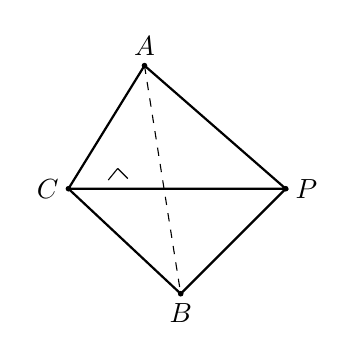
\begin{tikzpicture}[scale=0.92,>=stealth]
  \coordinate (C) at (0,0);
  \coordinate (P) at (3.0,0);
  \coordinate (A) at (1.05,1.7);
  \coordinate (B) at (1.55,-1.45);
  \draw[thick] (C)--(P);
  \draw[thick] (C)--(A)--(P)--cycle;
  \draw[thick] (C)--(B)--(P);
  \draw[dashed] (A)--(B);
  \draw (0.55,0.12)--(0.68,0.28);
  \draw (0.68,0.28)--(0.82,0.14);
  \fill (A) circle (1.1pt) node[above] {$A$};
  \fill (B) circle (1.1pt) node[below] {$B$};
  \fill (C) circle (1.1pt) node[left] {$C$};
  \fill (P) circle (1.1pt) node[right] {$P$};
\end{tikzpicture}
\end{center}
\nopagebreak[4]

\end{question}
\clearpage
\pdfbookmark[1]{参考答案与详细解析}{sec:s}
\Needspace{8\baselineskip}
\begin{center}{\Large\bfseries 参考答案与详细解析}\end{center}
\medskip
% answers.tex —— 1986 年·上海卷·理工农医类 · 参考答案与详细解析片段
% 由 tools/generate_projects.py 依来源总账自 1986/1986_数学真题_上海理_试题.md + 1986/1986_数学真题_上海理_解析正文.md + 1986/1986_数学真题_上海理_答案要点.md 生成，勿手改（改源 MD 后重跑）


\begin{gktip}
固定源第 3 页含答案表，第 4—5 页含解答。下列逐题推导由本库独立复算；第 9 题的幅角主值沿用固定源选项所反映的 $[0,2\pi)$ 约定。第 5 题按固定源解答，将 $k$ 视为实参数并把纯虚数理解为非零纯虚数。
\end{gktip}

\begin{answer}
\gksolhead{1}{}

\textbf{题目}：

（本题满分 40 分）本题共有 20 个小题，每一个小题都给出代号为 $A\text{、}B\text{、}C\text{、}D$ 的四个结论，其中有且只有一个结论是正确的。答题时，在答题纸上把代表正确结论代号的小圈按答题纸上的要求涂黑，每小题涂对得 2 分，不涂、涂错或涂黑的小圈数超过一个，则得零分。

（1） 平移坐标轴，把原点 $O(0,0)$ 移到 $O'(2,-1)$，则点 $(-1,-3)$ 在新坐标系中的坐标是\mbox{（　　）}

（A）$(3,2)$　　（B）$(-3,-2)$　　（C）$(-3,2)$　　（D）$(3,-2)$

（2） 下列三角关系式中不正确的是\mbox{（　　）}

（A）$\sin\alpha+\sin\beta=2\sin\frac{\beta+\alpha}{2}\cos\frac{\beta-\alpha}{2}$

（B）$\sin\alpha-\sin\beta=2\cos\frac{\beta+\alpha}{2}\sin\frac{\beta-\alpha}{2}$

（C）$\cos\alpha+\cos\beta=2\cos\frac{\beta+\alpha}{2}\cos\frac{\beta-\alpha}{2}$

（D）$\cos\alpha-\cos\beta=2\sin\frac{\beta+\alpha}{2}\sin\frac{\beta-\alpha}{2}$

（3） 在直角坐标系中，直线 $x+\sqrt3y+1=0$ 的倾角是\mbox{（　　）}

（A）$\frac\pi6$　　（B）$\frac\pi3$　　（C）$\frac{2\pi}3$　　（D）$\frac{5\pi}6$

（4） 函数 $y=2\operatorname{tg}\left(3x+\dfrac\pi6\right)$ 的最小正周期是\mbox{（　　）}

（A）$\frac\pi6$　　（B）$\frac\pi3$　　（C）$\frac\pi2$　　（D）$\frac{2\pi}3$

（5） 在空间中，下列命题中正确的是\mbox{（　　）}

（A）如果两直线 $a\text{、}b$ 与直线 $l$ 所成的角相等，那么 $a\parallel b$。

（B）如果两直线 $a\text{、}b$ 与平面 $\alpha$ 所成的角相等，那么 $a\parallel b$。

（C）如果直线 $l$ 与两平面 $\alpha\text{、}\beta$ 所成的角都是直角，那么 $\alpha\parallel\beta$。

（D）如果平面 $\gamma$ 与两平面 $\alpha\text{、}\beta$ 所成的二面角都是直二面角，那么 $\alpha\parallel\beta$。

（6） 当 $|x|\le1$ 时，$\arccos(-x)$ 等于\mbox{（　　）}

（A）$\pi-\arccos x$　　（B）$-\arccos x$　　（C）$\arccos x$　　（D）$\pi+\arccos x$

\Needspace{5\baselineskip}
（7） 极坐标方程

\nopagebreak[4]
\[
\rho=\frac5{2-4\cos\theta}
\]

所表示的曲线是\mbox{（　　）}

（A）椭圆　　（B）抛物线　　（C）双曲线　　（D）直线

（8） 下列双曲线方程中，以 $y=\pm\dfrac12x$ 为渐近线的是\mbox{（　　）}

（A）$\frac{x^2}{16}-\frac{y^2}{4}=1$

（B）$\frac{x^2}{4}-\frac{y^2}{16}=1$

（C）$\frac{x^2}{2}-y^2=1$

（D）$x^2-\frac{y^2}{2}=1$

（9） 复数 $\sqrt3-i$ 的幅角的主值是\mbox{（　　）}

（A）$\frac\pi6$　　（B）$\frac{5\pi}6$　　（C）$\frac{7\pi}6$　　（D）$\frac{11\pi}6$

（10） 等式 $\log_3x^2=2$ 成立是等式 $\log_3x=1$ 成立的\mbox{（　　）}

（A）充分但不是必要条件　　（B）必要但不是充分条件

（C）充分而且必要条件　　（D）既不充分又不必要的条件

（11） 在等比数列中，已知首项为 $\dfrac98$，末项为 $\dfrac13$，公比为 $\dfrac23$，则项数是\mbox{（　　）}

（A）3　　（B）4　　（C）5　　（D）6

（12） 已知定直线 $l$ 和 $l$ 外一定点 $A$，过点 $A$ 且与 $l$ 相切的圆的圆心轨迹是\mbox{（　　）}

（A）抛物线　　（B）双曲线　　（C）椭圆　　（D）直线

（13） 若 $\sin\dfrac\theta2=\dfrac35$，$\cos\dfrac\theta2=-\dfrac45$，则 $\theta$ 角的终边在\mbox{（　　）}

（A）第一象限　　（B）第二象限　　（C）第三象限　　（D）第四象限

（14） 下列不等式中正确的是\mbox{（　　）}

（A）$\sin\frac{5\pi}7>\sin\frac{4\pi}7$

（B）$\operatorname{tg}\frac{15\pi}8>\operatorname{tg}\left(-\frac\pi7\right)$

（C）$\sin\left(-\frac\pi5\right)>\sin\left(-\frac\pi6\right)$

（D）$\cos\left(-\frac{3\pi}5\right)>\cos\left(-\frac{9\pi}4\right)$

（15） 函数 $y=\lg\left(x+\sqrt{x^2+1}\right)$ 是\mbox{（　　）}

（A）奇函数而不是偶函数　　（B）偶函数而不是奇函数

（C）既不是奇函数也不是偶函数　　（D）既是奇函数又是偶函数

（16） $0<a<b<1$，下列不等式中正确的是\mbox{（　　）}

（A）$a^a<a^b$　　（B）$b^a<b^b$　　（C）$a^a<b^a$　　（D）$b^b<a^b$

（17） 正方体 $ABCD-A_1B_1C_1D_1$ 中，直线 $BC_1$ 与 $AC$\mbox{（　　）}

（A）相交且垂直　　（B）相交但不垂直

（C）异面且垂直　　（D）异面但不垂直

（18） 设复数 $z=a+bi$（$a,b\in\mathbb R$，且 $b\ne0$），则 $|z^2|$，$|z|^2$，$z^2$ 的关系是\mbox{（　　）}

（A）$|z^2|=|z|^2\ne z^2$　　（B）$|z^2|=|z|^2=z^2$

（C）$|z^2|\ne|z|^2=z^2$　　（D）$|z^2|\ne|z|^2\ne z^2$

（19） 过抛物线焦点 $F$ 的直线与抛物线相交于 $A\text{、}B$ 两点。若 $A\text{、}B$ 在抛物线准线上的射影分别是 $A_1\text{、}B_1$，则 $\angle A_1FB_1$ 等于\mbox{（　　）}

（A）$45^\circ$　　（B）$60^\circ$　　（C）$90^\circ$　　（D）$120^\circ$

\Needspace{5\baselineskip}
（20） 令

\nopagebreak[4]
\[
I=\{(x,y)\mid x,y\in\mathbb R\},
\]

\nopagebreak[4]
\[
A=\left\{(x,y)\middle|\frac{y-3}{x-2}=1,\ x,y\in\mathbb R\right\},
\qquad
B=\{(x,y)\mid y=x+1,\ x,y\in\mathbb R\},
\]

则 $\overline A\cap B$ 是\mbox{（　　）}

（A）$\overline A$　　（B）$B$　　（C）$\varnothing$　　（D）$\{(2,3)\}$

\Needspace{4\baselineskip}
\textbf{解析}

\gksubpart{（1）}

\Needspace{5\baselineskip}
新坐标原点为 $O'(2,-1)$，所以

\nopagebreak[4]
\[
x'=x-2,\qquad y'=y+1.
\]

点 $(-1,-3)$ 的新坐标为 $(-3,-2)$。

\gksubpart{（2）}

\Needspace{5\baselineskip}
正确的和差化积公式为

\nopagebreak[4]
\[
\sin\alpha-\sin\beta
=2\cos\frac{\alpha+\beta}{2}\sin\frac{\alpha-\beta}{2}.
\]

选项（B）把最后一个因子的符号写反，故不正确。

\gksubpart{（3）}

\Needspace{5\baselineskip}
直线斜率为 $-\frac1{\sqrt3}$，在 $[0,\pi)$ 内的倾角为

\nopagebreak[4]
\[
\frac{5\pi}{6}.
\]

\gksubpart{（4）}

\Needspace{5\baselineskip}
$\operatorname{tg}u$ 的周期是 $\pi$。对 $u=3x+\frac\pi6$，最小正周期为

\nopagebreak[4]
\[
\frac\pi3.
\]

\gksubpart{（5）}

\Needspace{5\baselineskip}
两直线与同一直线等角、与同一平面等角，都不能推出两直线平行；两个二面角为直二面角也不能推出两平面平行。若直线 $l$ 同时垂直于平面 $\alpha$ 和 $\beta$，则两平面的法线方向相同，从而

\nopagebreak[4]
\[
\alpha\parallel\beta.
\]

故选（C）。

\gksubpart{（6）}

\Needspace{5\baselineskip}
反余弦的值取在 $[0,\pi]$，且

\nopagebreak[4]
\[
\cos(\pi-\arccos x)=-x.
\]

\Needspace{5\baselineskip}
故

\nopagebreak[4]
\[
\arccos(-x)=\pi-\arccos x.
\]

\gksubpart{（7）}

\Needspace{5\baselineskip}
极坐标方程可写为

\nopagebreak[4]
\[
\rho=\frac{5/2}{1-2\cos\theta}.
\]

标准形式中的离心率为 $2>1$，所以图形是双曲线。

\gksubpart{（8）}

双曲线 $\frac{x^2}{a^2}-\frac{y^2}{b^2}=1$ 的渐近线为 $y=\pm\frac ba x$。选项（A）中 $a=4,b=2$，得到 $y=\pm\frac12x$。

\gksubpart{（9）}

\nopagebreak[4]
\[
\sqrt3-i
=2\left(\cos\frac{11\pi}{6}+i\sin\frac{11\pi}{6}\right).
\]

按固定源选项所采用的 $[0,2\pi)$ 约定，主值为 $\frac{11\pi}{6}$；按 $(-\pi,\pi]$ 约定则写作 $-\frac\pi6$。

\gksubpart{（10）}

$\log_3x^2=2$ 的解为 $x=\pm3$，$\log_3x=1$ 的解为 $x=3$。因此前一个等式是后一个等式成立的必要但不充分条件。

\gksubpart{（11）}

\nopagebreak[4]
\[
\frac13=\frac98\left(\frac23\right)^{n-1}
=\frac98\left(\frac23\right)^3
\]

给出 $n=4$。

\gksubpart{（12）}

\Needspace{5\baselineskip}
若动圆圆心为 $Q$，圆过定点 $A$ 且与定直线 $l$ 相切，则

\nopagebreak[4]
\[
QA=\operatorname{dist}(Q,l).
\]

这正是以 $A$ 为焦点、以 $l$ 为准线的抛物线定义。

\gksubpart{（13）}

\Needspace{5\baselineskip}
由半角公式

\nopagebreak[4]
\[
\sin\theta=-\frac{24}{25},\qquad
\cos\theta=\frac7{25}.
\]

所以 $\sin\theta<0,\cos\theta>0$，终边在第四象限。

\gksubpart{（14）}

\Needspace{5\baselineskip}
有

\nopagebreak[4]
\[
\operatorname{tg}\frac{15\pi}{8}
=\operatorname{tg}\left(-\frac\pi8\right).
\]

由于正切函数在相应区间上递增，且 $-\frac\pi8>-\frac\pi7$，所以（B）成立。

\gksubpart{（15）}

\Needspace{5\baselineskip}
令

\nopagebreak[4]
\[
f(x)=\lg\left(x+\sqrt{x^2+1}\right).
\]

\Needspace{5\baselineskip}
因为

\nopagebreak[4]
\[
\left(\sqrt{x^2+1}-x\right)
\left(\sqrt{x^2+1}+x\right)=1,
\]

\Needspace{5\baselineskip}
所以

\nopagebreak[4]
\[
f(-x)
=\lg\left(\sqrt{x^2+1}-x\right)
=-f(x).
\]

故 $f$ 是奇函数而不是偶函数。

\gksubpart{（16）}

\Needspace{5\baselineskip}
固定正指数 $a$ 时，$t^a$ 在 $t>0$ 上递增。由 $a<b$ 得

\nopagebreak[4]
\[
a^a<b^a,
\]

所以正确选项为（C）。

\gksubpart{（17）}

\Needspace{5\baselineskip}
取

\nopagebreak[4]
\[
A=(0,0,0),\quad B=(1,0,0),\quad
C=(1,1,0),\quad C_1=(1,1,1).
\]

直线 $AC$ 与 $BC_1$ 的方向向量分别可取 $(1,1,0)$ 和 $(0,1,1)$，内积为 $1$；同时两直线不相交，故它们异面但不垂直。

\gksubpart{（18）}

\Needspace{5\baselineskip}
模的乘法性质给出

\nopagebreak[4]
\[
|z^2|=|z|^2.
\]

\Needspace{5\baselineskip}
而

\nopagebreak[4]
\[
z^2=(a^2-b^2)+2abi.
\]

\Needspace{5\baselineskip}
若 $a\ne0$，则 $z^2$ 有非零虚部；若 $a=0$，则 $z^2=-b^2$，也不等于 $|z|^2=b^2$。因此

\nopagebreak[4]
\[
|z^2|=|z|^2\ne z^2.
\]

\gksubpart{（19）}

\Needspace{5\baselineskip}
设抛物线为 $y^2=4\lambda x$，焦点 $F=(\lambda,0)$，准线为 $x=-\lambda$。过焦点的弦上两点可参数化为

\nopagebreak[4]
\[
A=(\lambda t^2,2\lambda t),\qquad
B=(\lambda s^2,2\lambda s),
\]

\Needspace{5\baselineskip}
且 $ts=-1$。它们在准线上的射影满足

\nopagebreak[4]
\[
\overrightarrow{FA_1}=(-2\lambda,2\lambda t),\qquad
\overrightarrow{FB_1}=(-2\lambda,2\lambda s).
\]

\Needspace{5\baselineskip}
于是

\nopagebreak[4]
\[
\overrightarrow{FA_1}\cdot\overrightarrow{FB_1}
=4\lambda^2(1+ts)=0.
\]

故 $\angle A_1FB_1=90^\circ$。

\gksubpart{（20）}

\Needspace{5\baselineskip}
分式条件隐含 $x\ne2$。由

\nopagebreak[4]
\[
\frac{y-3}{x-2}=1
\]

\Needspace{5\baselineskip}
可知

\nopagebreak[4]
\[
A=\{(x,x+1)\mid x\in\mathbb R,\ x\ne2\}
=B\setminus\{(2,3)\}.
\]

\Needspace{5\baselineskip}
在全集 $I$ 中

\nopagebreak[4]
\[
\overline A\cap B=\{(2,3)\}.
\]

\gkanswer{答案（1）：B}

\gkanswer{答案（2）：B}

\gkanswer{答案（3）：D}

\gkanswer{答案（4）：B}

\gkanswer{答案（5）：C}

\gkanswer{答案（6）：A}

\gkanswer{答案（7）：C}

\gkanswer{答案（8）：A}

\gkanswer{答案（9）：D}

\gkanswer{答案（10）：B}

\gkanswer{答案（11）：B}

\gkanswer{答案（12）：A}

\gkanswer{答案（13）：D}

\gkanswer{答案（14）：B}

\gkanswer{答案（15）：A}

\gkanswer{答案（16）：C}

\gkanswer{答案（17）：D}

\gkanswer{答案（18）：A}

\gkanswer{答案（19）：C}

\gkanswer{答案（20）：D}

\end{answer}
\begin{answer}
\gksolhead{2}{}

\textbf{题目}：

（本题满分 30 分）本题共有 10 个小题，每一个小题满分 3 分，只要求直接写出结果。

\Needspace{5\baselineskip}
（1） 若三点 $P_1\text{、}P_2$ 和 $P$ 在一条直线上，点 $P_1$ 和点 $P_2$ 在直角坐标系中的坐标分别为 $(0,-6)$ 和 $(3,0)$，且

\nopagebreak[4]
\[
\frac{\overline{P_1P}}{\overline{PP_2}}=-\frac12,
\]

则点 $P$ 的坐标是 $\underline{\hspace{2em}}$。

（2） 正方体的全面积是 6，则其内切球的体积是 $\underline{\hspace{2em}}$。

\Needspace{5\baselineskip}
（3） 计算下式：

\nopagebreak[4]
\[
\lim_{n\to\infty}\frac{1+3+5+\cdots+(2n-1)}{n(n+1)}
=\underline{\hspace{2em}}\text{。}
\]

\Needspace{5\baselineskip}
（4） 求一次项系数：

\nopagebreak[4]
\[
\left(\sqrt[3]{x}-\frac1{\sqrt{x}}\right)^8
\]

的展开式中，$x$ 的一次项的系数是 $\underline{\hspace{2em}}$。

\Needspace{5\baselineskip}
（5） 不等式组

\nopagebreak[4]
\[
\begin{cases}
\sqrt{x^2-9}\le4,\\
x>0
\end{cases}
\]

的解是 $\underline{\hspace{2em}}$。

（6） 轴截面是等边三角形的圆锥，它的侧面展开图扇形的圆心角的弧度数等于 $\underline{\hspace{2em}}$。

（7） 用 1、2、3、4 四个数字组成没有重复数字的四位奇数的个数是 $\underline{\hspace{2em}}$。

\Needspace{5\baselineskip}
（8） 已知 $\cos\theta=-\dfrac35$ 且 $\pi<\theta<\dfrac{3\pi}2$，则

\nopagebreak[4]
\[
\operatorname{ctg}\left(\theta-\frac\pi4\right)=\underline{\hspace{2em}}\text{。}
\]

\Needspace{5\baselineskip}
（9） 函数

\nopagebreak[4]
\[
y=\log_2\left(\log_{\frac12}x\right)
\]

的定义域是 $\underline{\hspace{2em}}$。

\Needspace{5\baselineskip}
（10） 直线 $l$ 的参数方程为

\nopagebreak[4]
\[
\begin{cases}
x=3+\dfrac48t,\\
y=-2+\dfrac38t,
\end{cases}
\]

过点 $(4,-1)$ 且与 $l$ 平行的直线在 $y$ 轴上的截距是 $\underline{\hspace{2em}}$。

\Needspace{4\baselineskip}
\textbf{解析}

\gksubpart{（1）}

\Needspace{5\baselineskip}
令 $P=P_1+t(P_2-P_1)$，则有向线段比给出

\nopagebreak[4]
\[
\frac{t}{1-t}=-\frac12,
\]

\Needspace{5\baselineskip}
所以 $t=-1$，从而

\nopagebreak[4]
\[
P=(-3,-12).
\]

\gksubpart{（2）}

\Needspace{5\baselineskip}
设正方体棱长为 $s$，则 $6s^2=6$，故 $s=1$。内切球半径为 $\frac12$，其体积为

\nopagebreak[4]
\[
\frac43\pi\left(\frac12\right)^3=\frac\pi6.
\]

\gksubpart{（3）}

\Needspace{5\baselineskip}
前 $n$ 个奇数的和为 $n^2$，故

\nopagebreak[4]
\[
\lim_{n\to\infty}
\frac{1+3+\cdots+(2n-1)}{n(n+1)}
=\lim_{n\to\infty}\frac n{n+1}=1.
\]

\gksubpart{（4）}

\Needspace{5\baselineskip}
若从

\nopagebreak[4]
\[
\left(\sqrt[3]x-\frac1{\sqrt x}\right)^8
\]

\Needspace{5\baselineskip}
中取 $k$ 个第二项，则对应幂次为

\nopagebreak[4]
\[
\frac{8-k}{3}-\frac k2.
\]

\Needspace{5\baselineskip}
令其等于 $1$ 得 $k=2$，系数为

\nopagebreak[4]
\[
\binom82(-1)^2=28.
\]

\gksubpart{（5）}

\Needspace{5\baselineskip}
由根式定义域和不等式得

\nopagebreak[4]
\[
x^2-9\ge0,\qquad x^2-9\le16,\qquad x>0.
\]

\Needspace{5\baselineskip}
所以

\nopagebreak[4]
\[
3\le x\le5.
\]

\gksubpart{（6）}

\Needspace{5\baselineskip}
轴截面为等边三角形时，圆锥母线 $l$ 等于底面直径 $2r$。展开扇形的弧长为 $2\pi r$，所以圆心角为

\nopagebreak[4]
\[
\frac{2\pi r}{l}=\pi.
\]

\gksubpart{（7）}

\Needspace{5\baselineskip}
末位必须为 $1$ 或 $3$，有 2 种选法；其余三位有 $3!$ 种排列，故

\nopagebreak[4]
\[
2\cdot3!=12.
\]

\gksubpart{（8）}

\Needspace{5\baselineskip}
在第三象限中 $\sin\theta=-\frac45$，代入余切差角公式：

\nopagebreak[4]
\[
\operatorname{ctg}\left(\theta-\frac\pi4\right)
=\frac{\cos\theta+\sin\theta}{\sin\theta-\cos\theta}
=\frac{-3/5-4/5}{-4/5+3/5}=7.
\]

\gksubpart{（9）}

\Needspace{5\baselineskip}
外层对数要求

\nopagebreak[4]
\[
\log_{\frac12}x>0.
\]

由于底数小于 1，这等价于 $0<x<1$。

\gksubpart{（10）}

\Needspace{5\baselineskip}
参数方程的方向向量可取 $\left(\frac48,\frac38\right)$，所以直线斜率为 $\frac34$。过 $(4,-1)$ 的平行线为

\nopagebreak[4]
\[
y+1=\frac34(x-4).
\]

令 $x=0$，得到其在 $y$ 轴上的截距为 $-4$。

\gkanswer{答案（1）：$(-3,-12)$}

\gkanswer{答案（2）：$\dfrac\pi6$}

\gkanswer{答案（3）：$1$}

\gkanswer{答案（4）：$28$（或 $C_8^2$）}

\gkanswer{答案（5）：$3\le x\le5$}

\gkanswer{答案（6）：$\pi$}

\gkanswer{答案（7）：$12$}

\gkanswer{答案（8）：$7$}

\gkanswer{答案（9）：$(0,1)$}

\gkanswer{答案（10）：$-4$}

\end{answer}
\begin{answer}
\gksolhead{3}{}

\textbf{题目}：

\Needspace{5\baselineskip}
（本题满分 7 分）设数列 $\{a_n\}$ 的前 $n$ 项和为

\nopagebreak[4]
\[
S_n=n^2+2n+4\qquad(n\in\mathbb N),
\]

（1） 写出这个数列的前 $3$ 项 $a_1,a_2,a_3$；

（2） 证明：数列 $\{a_n\}$ 除去首项后所成的数列 $a_2,a_3,a_4,\ldots$ 是等差数列。

\Needspace{4\baselineskip}
\textbf{解析}

\gksubpart{（1）}

\Needspace{5\baselineskip}
由

\nopagebreak[4]
\[
S_n=n^2+2n+4
\]

\Needspace{5\baselineskip}
得到

\nopagebreak[4]
\[
a_1=S_1=7,
\]

\nopagebreak[4]
\[
a_2=S_2-S_1=5,\qquad
a_3=S_3-S_2=7.
\]

\gksubpart{（2）}

\Needspace{5\baselineskip}
对 $n\ge2$，

\nopagebreak[4]
\[
\begin{aligned}
a_n
&=S_n-S_{n-1}\\
&=n^2+2n+4-\bigl((n-1)^2+2(n-1)+4\bigr)\\
&=2n+1.
\end{aligned}
\]

\Needspace{5\baselineskip}
因此

\nopagebreak[4]
\[
a_{n+1}-a_n=2\qquad(n\ge2),
\]

数列 $a_2,a_3,a_4,\ldots$ 是公差为 2 的等差数列。

\gkanswer{答案（1）：$a_1=7,\ a_2=5,\ a_3=7$}

\gkanswer{答案（2）：见解析正文。}

\end{answer}
\begin{answer}
\gksolhead{4}{}

\textbf{题目}：

\Needspace{5\baselineskip}
（本题满分 7 分）设 $x>0,\ y>0$，证明不等式

\nopagebreak[4]
\[
(x^2+y^2)^{1/2}>(x^3+y^3)^{1/3}.
\]

\Needspace{4\baselineskip}
\textbf{解析}

\Needspace{5\baselineskip}
由于两边均为正数，可以比较六次方：

\nopagebreak[4]
\[
\begin{aligned}
(x^2+y^2)^3-(x^3+y^3)^2
&=x^2y^2(3x^2-2xy+3y^2)\\
&=x^2y^2\left[3\left(x-\frac y3\right)^2
+\frac83y^2\right]>0.
\end{aligned}
\]

\Needspace{5\baselineskip}
故

\nopagebreak[4]
\[
(x^2+y^2)^{1/2}>(x^3+y^3)^{1/3}.
\]

\gkanswer{答案：见解析正文。}

\end{answer}
\begin{answer}
\gksolhead{5}{}

\textbf{题目}：

\Needspace{5\baselineskip}
（本题满分 12 分）本题共有 2 个小题，每个小题满分 6 分。已知 $k$ 为实数，复数

\nopagebreak[4]
\[
z=\cos\theta+i\sin\theta.
\]

（1） 当 $\theta$ 和 $k$ 分别取何值时，$z^3+k\overline z^{\,3}$ 是纯虚数；

（2） 当 $\theta$ 变化时，求 $|z^3+k\overline z^{\,3}|$ 的最大值和最小值。

\Needspace{4\baselineskip}
\textbf{解析}

\gksubpart{（1）}

\Needspace{5\baselineskip}
因 $|z|=1$，有

\nopagebreak[4]
\[
z^3=\cos3\theta+i\sin3\theta,\qquad
\overline z^{\,3}=\cos3\theta-i\sin3\theta.
\]

\Needspace{5\baselineskip}
所以

\nopagebreak[4]
\[
z^3+k\overline z^{\,3}
=(1+k)\cos3\theta+i(1-k)\sin3\theta.
\]

\Needspace{5\baselineskip}
若按源解答把纯虚数限定为非零纯虚数，则须满足

\nopagebreak[4]
\[
(1+k)\cos3\theta=0,\qquad
(1-k)\sin3\theta\ne0.
\]

\Needspace{5\baselineskip}
因此参数条件可写为

\nopagebreak[4]
\[
\boxed{
\begin{cases}
k=-1,\quad \theta\ne\dfrac{n\pi}{3};\\[4pt]
\text{\text{或} }k\ne1,\quad
\theta=\dfrac\pi6+\dfrac{n\pi}{3},
\end{cases}
\quad n\in\mathbb Z.}
\]

\gksubpart{（2）}

\Needspace{5\baselineskip}
当 $\theta$ 变化时，

\nopagebreak[4]
\[
\begin{aligned}
|z^3+k\overline z^{\,3}|^2
&=(1+k)^2\cos^23\theta+(1-k)^2\sin^23\theta\\
&=1+k^2+2k\cos6\theta.
\end{aligned}
\]

\Needspace{5\baselineskip}
故最大值和最小值分别为

\nopagebreak[4]
\[
\boxed{1+|k|},\qquad
\boxed{|1-|k||}.
\]

\gkanswer{答案（1）：见解析正文。}

\gkanswer{答案（2）：最大值 $1+|k|$，最小值 $|1-|k||$}

\end{answer}
\begin{answer}
\gksolhead{6}{}

\textbf{题目}：

\Needspace{5\baselineskip}
（本题满分 12 分）如果抛物线

\nopagebreak[4]
\[
y^2=px
\]

\Needspace{5\baselineskip}
和圆

\nopagebreak[4]
\[
(x-2)^2+y^2=3
\]

相交，它们在 $x$ 轴上方的交点为 $A$ 和 $B$，那么当 $p$ 为何值时，线段 $AB$ 的中点 $M$ 在直线 $y=x$ 上。
\nopagebreak[4]
\begin{center}% 1986 年上海卷理工农医类第 6 题：抛物线与圆
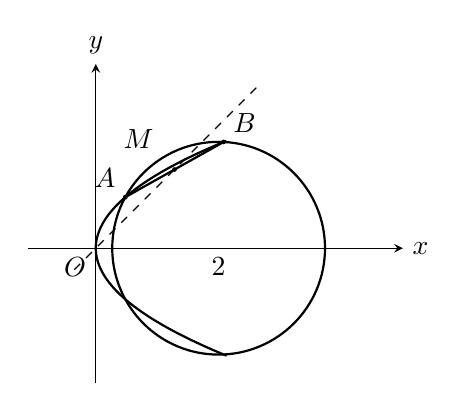
\begin{tikzpicture}[scale=0.78,>=stealth]
  \draw[->] (-1.1,0)--(5.0,0) node[right] {$x$};
  \draw[->] (0,-2.2)--(0,3.0) node[above] {$y$};
  \draw[thick] (2,0) circle (1.732);
  \draw[thick,domain=-1.75:1.75,samples=100]
    plot ({\x*\x/1.438},{\x});
  \draw[dashed] (-0.35,-0.35)--(2.65,2.65);
  \draw[thick] (0.480,0.831)--(2.081,1.730);
  \fill (0.480,0.831) circle (1.1pt) node[above left] {$A$};
  \fill (2.081,1.730) circle (1.1pt) node[above right] {$B$};
  \fill (1.281,1.281) circle (1.1pt) node[above left,xshift=-4pt,yshift=4pt] {$M$};
  \node[below left] at (0,0) {$O$};
  \node[below] at (2,0) {$2$};
\end{tikzpicture}
\end{center}
\nopagebreak[4]
\Needspace{4\baselineskip}
\textbf{解析}

\Needspace{5\baselineskip}
联立

\nopagebreak[4]
\[
y^2=px,\qquad (x-2)^2+y^2=3
\]

\Needspace{5\baselineskip}
得

\nopagebreak[4]
\[
x^2+(p-4)x+1=0.
\]

\Needspace{5\baselineskip}
若两个交点横坐标为 $x_1,x_2$，则

\nopagebreak[4]
\[
x_1+x_2=4-p,\qquad x_1x_2=1.
\]

\Needspace{5\baselineskip}
两点在 $x$ 轴上方，所以

\nopagebreak[4]
\[
y_1+y_2
=\sqrt{p(x_1+x_2)+2p\sqrt{x_1x_2}}
=\sqrt{6p-p^2}.
\]

\Needspace{5\baselineskip}
中点为

\nopagebreak[4]
\[
M=\left(\frac{4-p}{2},\frac{\sqrt{6p-p^2}}2\right).
\]

\Needspace{5\baselineskip}
令 $M$ 在 $y=x$ 上，得到

\nopagebreak[4]
\[
6p-p^2=(4-p)^2,
\]

\Needspace{5\baselineskip}
即

\nopagebreak[4]
\[
p^2-7p+8=0.
\]

\Needspace{5\baselineskip}
两个根为 $\frac{7\pm\sqrt{17}}2$。因 $x_M=(4-p)/2\ge0$，舍去大根，故

\nopagebreak[4]
\[
p=\frac{7-\sqrt{17}}2.
\]

\gkanswer{答案：$\dfrac{7-\sqrt{17}}2$}

\end{answer}
\begin{answer}
\gksolhead{7}{}

\textbf{题目}：

（本题满分 12 分）已知直角三角形 $ABC$ 的两直角边 $AC=2$，$BC=3$，$P$ 为斜边 $AB$ 上一点（图 1）。现沿 $CP$ 将此直角三角形折成直二面角 $A\mathbin{-}CP\mathbin{-}B$，当 $AB=\sqrt7$ 时，求二面角 $P\mathbin{-}AC\mathbin{-}B$ 的大小（图 2）。
\nopagebreak[4]
\begin{center}% 1986 年上海卷理工农医类第 7 题图 1：折叠前的直角三角形
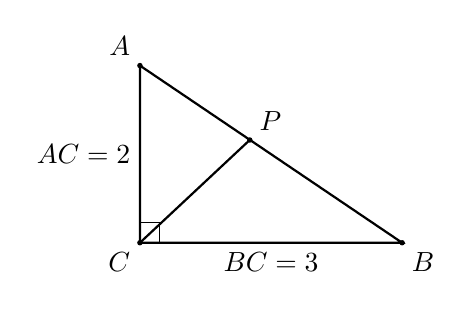
\begin{tikzpicture}[scale=0.9,>=stealth]
  \coordinate (C) at (0,0);
  \coordinate (A) at (0,2.5);
  \coordinate (B) at (3.7,0);
  \coordinate (P) at (1.55,1.45);
  \draw[thick] (A)--(C)--(B)--cycle;
  \draw[thick] (C)--(P);
  \draw (0,0.28)--(0.28,0.28)--(0.28,0);
  \fill (A) circle (1.1pt) node[above left] {$A$};
  \fill (B) circle (1.1pt) node[below right] {$B$};
  \fill (C) circle (1.1pt) node[below left] {$C$};
  \fill (P) circle (1.1pt) node[above right] {$P$};
  \node[left] at (0,1.25) {$AC=2$};
  \node[below] at (1.85,0) {$BC=3$};
\end{tikzpicture}
\end{center}
\nopagebreak[4]
\nopagebreak[4]
\begin{center}% 1986 年上海卷理工农医类第 7 题图 2：沿 CP 折成直二面角
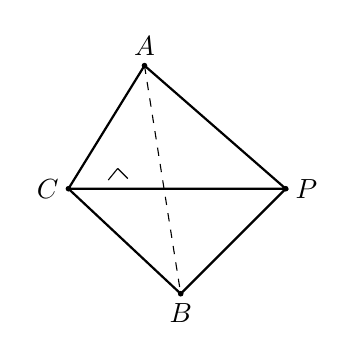
\begin{tikzpicture}[scale=0.92,>=stealth]
  \coordinate (C) at (0,0);
  \coordinate (P) at (3.0,0);
  \coordinate (A) at (1.05,1.7);
  \coordinate (B) at (1.55,-1.45);
  \draw[thick] (C)--(P);
  \draw[thick] (C)--(A)--(P)--cycle;
  \draw[thick] (C)--(B)--(P);
  \draw[dashed] (A)--(B);
  \draw (0.55,0.12)--(0.68,0.28);
  \draw (0.68,0.28)--(0.82,0.14);
  \fill (A) circle (1.1pt) node[above] {$A$};
  \fill (B) circle (1.1pt) node[below] {$B$};
  \fill (C) circle (1.1pt) node[left] {$C$};
  \fill (P) circle (1.1pt) node[right] {$P$};
\end{tikzpicture}
\end{center}
\nopagebreak[4]
\Needspace{4\baselineskip}
\textbf{解析}

\Needspace{5\baselineskip}
设 $\alpha=\angle BCP$。在折叠后的两个互相垂直平面内，过 $A\text{、}B$ 分别作 $CP$ 的垂线 $AD\text{、}BE$，则

\nopagebreak[4]
\[
CD=2\sin\alpha,\quad AD=2\cos\alpha,
\]

\nopagebreak[4]
\[
CE=3\cos\alpha,\quad BE=3\sin\alpha.
\]

\Needspace{5\baselineskip}
因此

\nopagebreak[4]
\[
\begin{aligned}
AB^2
&=(CE-CD)^2+AD^2+BE^2\\
&=(3\cos\alpha-2\sin\alpha)^2
+(2\cos\alpha)^2+(3\sin\alpha)^2\\
&=13-6\sin2\alpha.
\end{aligned}
\]

按题设折叠后的空间距离 $AB=\sqrt7$，故 $\sin2\alpha=1$。由于 $0<\alpha<\frac\pi2$，所以 $\alpha=45^\circ$，且 $\angle ACP=45^\circ$。

\Needspace{5\baselineskip}
折叠后的三角形 $ABC$ 的三边为 $2,3,\sqrt7$，由余弦定理

\nopagebreak[4]
\[
\cos\angle ACB
=\frac{2^2+3^2-7}{2\cdot2\cdot3}
=\frac12,
\]

\Needspace{5\baselineskip}
得到 $\angle ACB=60^\circ$。在包含 $AC$ 的两个截面内，过 $A$ 作垂直于 $AC$ 的线段 $AH\text{、}AK$，则

\nopagebreak[4]
\[
AH=AC\tan45^\circ=2,\qquad
AK=AC\tan60^\circ=2\sqrt3.
\]

\Needspace{5\baselineskip}
二面角 $P\mathbin{-}AC\mathbin{-}B$ 的平面角满足

\nopagebreak[4]
\[
\cos\angle HAK=\frac{AH}{AK}
=\frac1{\sqrt3}=\frac{\sqrt3}{3}.
\]

\Needspace{5\baselineskip}
所以所求二面角为

\nopagebreak[4]
\[
\arccos\frac{\sqrt3}{3}.
\]

\gkanswer{答案：$\arccos\dfrac{\sqrt3}{3}$}

\end{answer}
\end{document}
